\documentclass[11pt]{article}
\ProvidesPackage{calcpractices}[2026/05/14 AP Calculus BC shared preamble]
\usepackage[margin=1in]{geometry}
\usepackage{fancyhdr}
\usepackage{amsmath}
\usepackage{tikz}
\usepackage{pgfplots}
\usepackage{multicol}
\pgfplotsset{compat=1.18}

\pagestyle{fancy}
\fancyhf{}
\fancyhead[L]{AP Calculus BC}
\fancyhead[R]{Practice}
\fancyfoot[C]{\thepage}

\newcommand{\emptygraph}{
    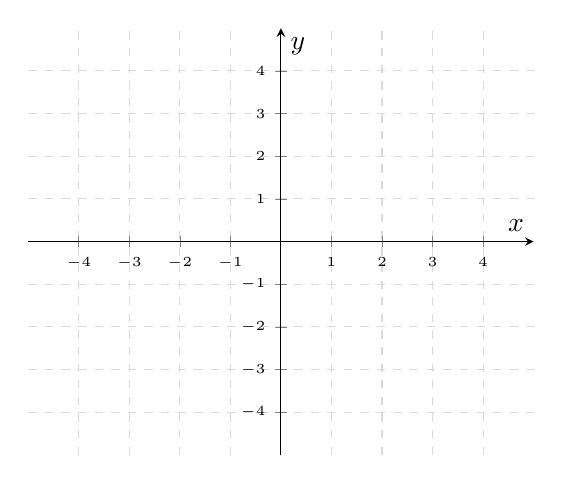
\begin{tikzpicture}
        \begin{axis}[
            axis lines = middle,
            grid = both,
            width=8cm,
            height=7cm,
            xmin=-5, xmax=5,
            ymin=-5, ymax=5,
            xtick={-4,-3,...,4},
            ytick={-4,-3,...,4},
            xlabel={$x$},
            ylabel={$y$},
            tick label style={font=\tiny},
            grid style={dashed, gray!30}
        ]
        \end{axis}
    \end{tikzpicture}
}

\newcommand{\smallgraph}{
    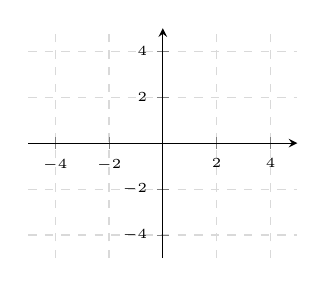
\begin{tikzpicture}
        \begin{axis}[
            axis lines = middle,
            grid = both,
            width=5cm,
            height=4.5cm,
            xmin=-5, xmax=5,
            ymin=-5, ymax=5,
            xtick={-4,-2,0,2,4},
            ytick={-4,-2,0,2,4},
            tick label style={font=\tiny},
            grid style={dashed, gray!30}
        ]
        \end{axis}
    \end{tikzpicture}
}

\fancyhead[C]{1.4 Parametric Equations}

\begin{document}

\noindent Use a calculator to graph the following. Show the approximate window size in your sketch. Give a parameter interval that traces the curve \textbf{exactly once}, and show the starting and finishing point.

\begin{enumerate}

\begin{multicols}{2}
    \item $\displaystyle x = 3\sin(2t),\quad \\y = 1.5\cos(t)$\\[1ex]\smallgraph
    \item $\displaystyle x = \sin^3 t,\quad \\y = \cos^3 t$\\[1ex]\smallgraph
\end{multicols}

\begin{multicols}{2}
    \item $\displaystyle x = 7\sin t - \sin(7t),\quad \\y = 7\cos t - \cos(7t)$\\[1ex]\smallgraph
    \item $\displaystyle x = 12\sin(t) - 3\sin(6t),\quad \\y = 12\cos(t) + 3\cos(6t)$\\[1ex]\smallgraph
\end{multicols}

\vspace{1ex}

\noindent For the following, a parameterization is given for a curve. Graph the curve. Show the initial and terminal points, if any. Indicate the direction in which the curve is traced. Find a Cartesian equation for the curve that contains the parameterized curve. Show what portion of the graph of the Cartesian equation is traced by the parameterized curve.

\begin{multicols}{2}
    \item $\displaystyle x = -\sqrt{t},\quad y = t,\quad t \ge 0$\\[1ex]\smallgraph
    \item $\displaystyle x = \sec^2 t - 1,\quad y = \tan t,\quad -\dfrac{\pi}{2} < t < \dfrac{\pi}{2}$\\[1ex]\smallgraph
\end{multicols}

\begin{multicols}{2}
    \item $\displaystyle x = \sin(2\pi t),\quad y = \cos(2\pi t),\quad 0 \le t \le 1$\\[1ex]\smallgraph
    \item $\displaystyle x = 1 - t,\quad y = 1 + t,\quad -\infty < t < \infty$\\[1ex]\smallgraph
\end{multicols}

\begin{multicols}{2}
    \item $\displaystyle x = t^2,\quad y = \sqrt{4 - t^2},\quad 0 \le t \le 2$\\[1ex]\smallgraph
    \item $\displaystyle x = t^2 - 3,\quad y = t,\quad t \le 0$\\[1ex]\smallgraph
\end{multicols}

\vspace{2ex}

\noindent Find a parameterization of the curve.

\item The line segment with endpoints $\displaystyle (-1, -3)$ and $\displaystyle (4, 1)$.

\vspace{6ex}

\item The line segment with endpoints $\displaystyle (-1, 3)$ and $\displaystyle (3, -2)$.

\vspace{6ex}

\item The lower half of the parabola $\displaystyle x - 1 = y^2$.

\vspace{6ex}

\item The left half of the parabola $\displaystyle y = x^2 + 2x$.

\vspace{6ex}

\item Graph the following: $\displaystyle x = 3 - |t|,\quad y = t - 1,\quad -5 \le t \le 5$. \textbf{(Note the domain of $t$.)}

\emptygraph

\noindent Find the values of $t$ that produce the portion of the graph that is in Quadrant I. Repeat for Quadrants II, III, and IV.

\vspace{4cm}

\newpage

\noindent For the following, find a parameterization for the part of the graph in Quadrant I.

\begin{multicols}{2}
    \item $\displaystyle y = x^2 + 2x + 2$\\[5ex]
    \item $\displaystyle y = \sqrt{x + 3}$\\[5ex]
\end{multicols}

\item Find parameterizations to model the motion of a particle that starts at $\displaystyle (a, 0)$ and traces the circle $\displaystyle x^2 + y^2 = a^2$, $a > 0$, as indicated.\\[1ex]

\noindent Once clockwise:
\vspace{2cm}

\noindent Once counterclockwise:
\vspace{2cm}

\noindent Twice clockwise:
\vspace{2cm}

\item Find parameterizations to model the motion of a particle that starts at $\displaystyle (-a, 0)$ and traces the ellipse $\displaystyle \left(\dfrac{x}{a}\right)^2 + \left(\dfrac{y}{b}\right)^2 = 1$, $a > 0$, $b > 0$, as indicated.\\[1ex]

\noindent Once clockwise:
\vspace{2cm}

\noindent Once counterclockwise:
\vspace{2cm}

\noindent Twice counterclockwise:
\vspace{2cm}

\end{enumerate}

\end{document}
